\section{La partícula libre}
\label{La partícula libre}

En el contexto de la mecánica cuántica, las partículas cuánticas muestran características tanto de ondas como de 
partículas (clásicamente hablando). Es por eso que es necesario implementar un esquema matemático adecuado que englobe 
ambas características de forma simultánea y satisfactoria.\\
En la física clásica, una partícula está bien localizada en el espacio, dado que su posición y velocidad pueden ser 
calculadas simultáneamente con precisión arbitraria. Mientras que en la mecánica cuántica, una partícula se describe 
mediante una función de onda correspondiente a la onda de materia asociada con la partícula \emph{(Hipótesis de De Broglie)}. 
Dada la situación, una partícula que sea localizable en una cierta región del espacio puede ser descrita por una onda de materia 
cuya amplitud sea grande en esa región y cero fuera de ella. De esta manera, la onda de materia será localizada dentro 
de la región del espacio donde la partícula esté físicamente confinada.\\
Una función de onda localizable es llamada un \emph{paquete de ondas}. Un paquete de ondas consiste entonces de una 
superposición de un grupo de ondas de ligeramente distintas longitudes de onda, con fases y amplitudes tales que 
interfieran constructivamente dentro de una pequeña región del espacio y destructivamente fuera de ella.\\

Matemáticamente es posible llevar a cabo dicha superposición de ondas gracias a la \emph{Transformada de Fourier}. Por 
simplicidad, se considerará un paquete de ondas unidimensional con la intención de describir a una partícula "clásica" 
confinada a una región unidimensional.\\
Es posible construir $\Psi(x,t)$ superponiendo ondas planas viajeras de distintas frecuencias (o longitudes de onda):

\begin{equation}
    \Psi(x,t) = \frac{1}{\sqrt{2\pi}} \int_{-\infty}^{\infty} \phi(k)e^{i(kx-\omega t)}\,dk
\end{equation}

Donde $\phi(k)$ es la amplitud del paquete de ondas.\\
Es importante tomar en cuenta que $\omega$ no es una constante dentro de la integral, de hecho $\omega$ es una función de 
$k$, i.e. $\omega=\omega(k)$.\\
De las relaciones de De Broglie:
\begin{equation*}
    \omega = \frac{E}{\hbar} = \frac{p^2/2m}{\hbar} = \frac{(\hbar k)^2}{2m\hbar} = \frac{\hbar k^2}{2m}
\end{equation*}

El objetivo es hallar la evolución temporal de este paquete de ondas. Para lograr esto, se analiza primero la forma del 
paquete en un tiempo dado. Por decir, en $t=0$:

\begin{equation}
    \Psi(0,t) = \psi_{0}(x) = \frac{1}{\sqrt{2\pi}} \int_{-\infty}^{\infty} \phi(k)e^{ikx}\,dk
\end{equation}

De lo revisado en la \emph{sección 2}, se pueden hallar las amplitudes $\phi(k)$ si se aplica una transformada de Fourier
a $\psi_{0}(x)$:

\begin{equation}
    \phi(k) = \frac{1}{\sqrt{2\pi}} \int_{-\infty}^{\infty} \psi_{0}(x)e^{-ikx}\,dx
\end{equation}

De esta manera, si se conoce la forma inicial de la función de onda, será posible encontrar las amplitudes $\phi(k)$ con
$(11)$, y finalmente la función de onda con su dependencia temporal en $(9)$. Más formalmente se puede resumir este 
algoritmo como trasladar la función de onda $\psi_{0}(x)$ del \emph{espacio de posiciones} a su representación $\phi(k)$ 
en el \emph{espacio-k}, también conocido como \emph{espacio de momentos}, para finalmente volver al \emph{espacio-x} 
agregando la dependencia temporal de la función de onda. Cabe destacar que tanto $\psi_{0}(x)$ como $\phi(k)$ contienen 
la misma información y son descripciones igualmente válidas para un estado cuántico.\\

Considérese por ejemplo a una partícula libre con la función de onda inicial:
\begin{equation}
    \Psi(x,0) = Ae^-ax^2
\end{equation}
Donde $A$ y $a$ son constantes (a es real y positiva).\\

Lo primero que se busca hacer es normalizar la función de onda para que su modulo al cuadrado adquiera un sentido 
estadístico apropiado de acuerdo con la interpretación de Born.
\begin{align*}
    \int_{-\infty}^{\infty} \lvert\Psi(x,0)\rvert^2\,dx &= \lvert A \rvert^2 \int_{-\infty}^{\infty} e^{-2ax^2}\,dx \\
    &= 2\lvert A \rvert^2 \int_{0}^{\infty} e^{-2ax^2}\,dx
\end{align*}

Efectuando cambios de variable apropiados:
\begin{align*}
    \int_{-\infty}^{\infty} \lvert\Psi(x,0)\rvert^2\,dx &= \frac{1}{\sqrt{2a}} \lvert A \rvert^2 \int_{0}^{\infty} t^{-1/2}e^{-t}\,dt \\
    &= \frac{1}{\sqrt{2a}} \lvert A \rvert^2 \,\Gamma(\frac{1}{2}) = \sqrt{\frac{\pi}{2a}} \lvert A \rvert^2
\end{align*}

De la condición de normalización:
\begin{gather*}
    \int_{-\infty}^{\infty} \lvert\Psi(x,0)\rvert^2\,dx = \sqrt{\frac{\pi}{2a}} \lvert A \rvert^2 = 1 \\
    \therefore A = \left (\frac{2a}{\pi}\right )^{1/4}
\end{gather*}

Una vez normalizada la función de onda inicial $\Psi(x,0) = \left (\frac{2a}{\pi}\right )^{1/4} e^{-ax^2}$, se obtiene 
$\phi(k)$ con la Transformada de Fourier según la ec. $(11)$:

\begin{align*}
    \phi(k) &= \frac{1}{\sqrt{2\pi}} \int_{-\infty}^{\infty} \psi_{0}(x)e^{-ikx}\,dx \\
    &= \left(\frac{a}{2\pi^3}\right)^{1/4} \int_{-\infty}^{\infty} e^{-(ax^2+ikx)}\,dx
\end{align*}

Con el apoyo de la librería \emph{Scipy} utilizando la función de transformada de Fourier, se obtiene el resultado:
\begin{equation}
    \phi(k) = \frac{1}{(2\pi a)^{1/4}} e^{-\frac{k^2}{4a}}
\end{equation}

Fijando un valor para $a$ de $a=\frac{1}{2\pi}$, se puede obtener gráficamente un representación para esta función de 
onda en el espacio de frecuencias:\\

\begin{figure}[H]
    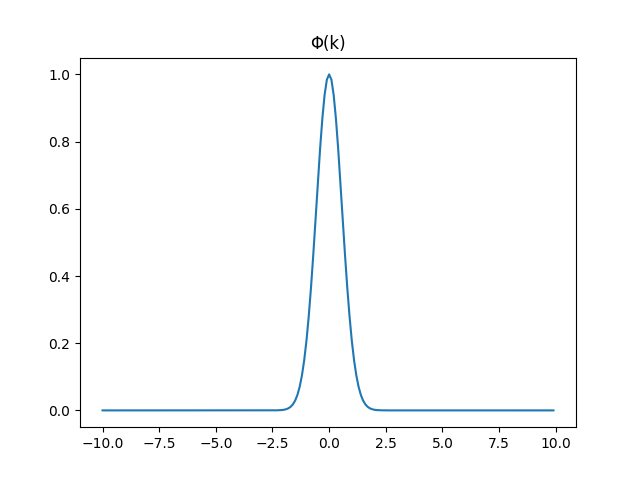
\includegraphics[scale=0.45]{imagenes/graficas_particulalibre/phi(k).png}
    \caption{\emph{$a = \frac{1}{2\pi}$}}
\end{figure}

Luego, de la ec. $(9)$:
\begin{align*}
    \Psi(x,t) &= \frac{1}{\sqrt{2\pi}} \int_{-\infty}^{\infty} \phi(k)e^{i(kx-\frac{\hbar k^2}{2m} t)}\,dk \\
    &= \frac{1}{(8\pi^3 a)^{1/4}} \int_{-\infty}^{\infty} e^{-\left[ \left( \frac{1}{4a}+\frac{i\hbar}{2m}t \right)k^2 - ixk\right]} \,dk
\end{align*}

Evidentemente esta es una integral algo laboriosa de hacer, así que se recurre una vez más a la librería \emph{Scipy}, 
utilizando esta vez la función de cálculo de integrales.\\
Se obtiene así la expresión general para la función de onda:
\begin{equation*}
    \Psi(x,t) = \left( \frac{2a}{\pi} \right)^{1/4} \frac{1}{\sqrt{1+\frac{2i\hbar a}{m}t}} e^{-\frac{ax^2}{1+\frac{2i\hbar a}{m}t}}
\end{equation*}

O de forma más simplificada haciendo\\ $\theta=\frac{2\hbar a}{m}t$:
\begin{equation}
    \Psi(x,t) = \left( \frac{2a}{\pi} \right)^{1/4} \frac{1}{\sqrt{1+i\theta}} e^{-\frac{ax^2}{1+i\theta}}
\end{equation}

Si suponemos que esta función de onda es asociada a un electrón, cuya masa es $m=9.11\times10^{-31} kg$; se puede 
representar gráficamente haciendo $a=\frac{1}{2\pi}$ (para conservar coherencia con la gráfica anterior) 
y tomando su función de onda inicial $\Psi(x,0)$:\\

\begin{figure}[H]
    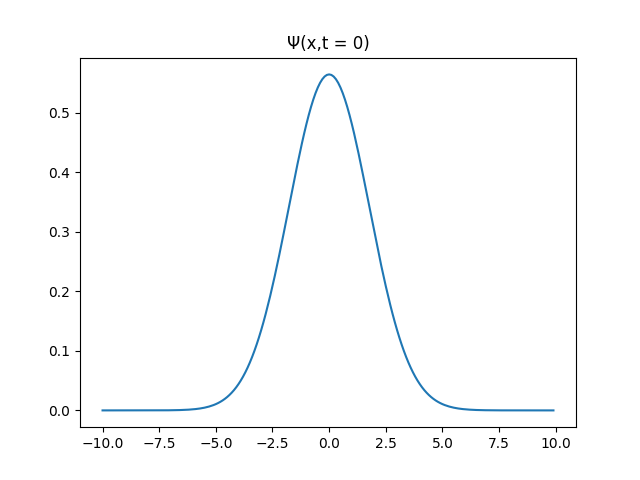
\includegraphics[scale=0.45]{imagenes/graficas_particulalibre/psi(x,t).png}
    \caption{\emph{$a = \frac{1}{2\pi}, t = 0$}}
\end{figure}

Se observa que se satisfacen las condiciones necesarias para una función de onda, i.e. la continuidad de $\Psi(x,t)$, 
así como en su derivada posicional de primer orden y la condición de que cuando $x\rightarrow\pm\infty$, $\Psi(x,t)=0$.\\

Ya obtenida la función de onda que describe a esta partícula, el verdadero sentido físico se adquiere al obtener el 
módulo al cuadrado de la antedicha:
\begin{equation*}
    \lvert\Psi(x,t)\rvert^2 = \Psi*\Psi = \sqrt{\frac{2a}{\pi}} \frac{1}{\sqrt{1+\theta^2}} e^{-\frac{2ax^2}{1+\theta^2}}
\end{equation*}

Esta función representa ahora una densidad de probabilidad. Más concretamente, la probabilidad de localizar al electrón 
en una región del espacio $x$, a un determinado tiempo $t$. Y si se define $\omega=\sqrt{\frac{a}{1+\theta^2}}$, se puede 
expresar de forma más simplificada:
\begin{equation}
    \rho(x,t) = \lvert\Psi(x,t)\rvert^2 = \sqrt{\frac{2}{\pi}} \omega e^{-2\omega^2x^2}
\end{equation}

\begin{figure}[H]
    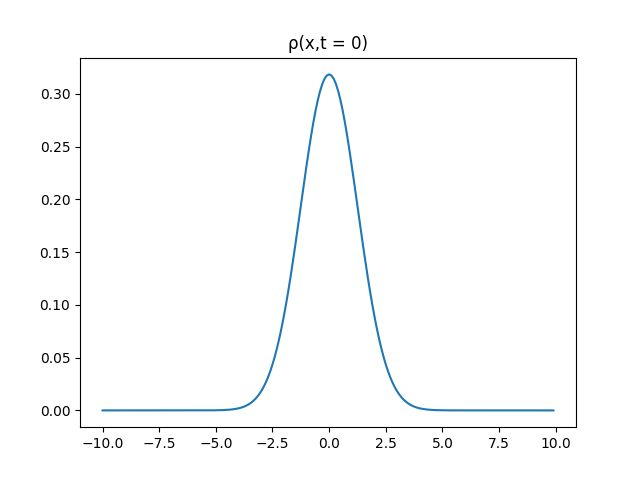
\includegraphics[scale=0.45]{imagenes/graficas_particulalibre/rho(x,t).png}
    \caption{\emph{$a = \frac{1}{2\pi}, t = 0$}}
\end{figure}

Ya sea a partir la función $\rho(x,t)$ o la misma gráfica, se observa la distribución gaussiana que tiene este electrón. 
Siendo así para cualquier tiempo arbitrario $t=t_{0}$ más probable de detectarlo en posiciones cercanas al origen, y mucho 
menos probable en posiciones alejadas de éste.